\documentclass[11p]{article}
% Packages
\usepackage{amsmath}
\usepackage{graphicx}
\usepackage[swedish]{babel}
\usepackage[
    backend=biber,
    style=authoryear-ibid,
    sorting=ynt
]{biblatex}
\usepackage[utf8]{inputenc}
\usepackage[T1]{fontenc}
%Källor
\graphicspath{ {./images/} }

\title{Labrapprt \\ \small Fysik 1}
\author{Nova Lindberg }
\date{\today}

\begin{document}

    \begin{titlepage}
        \begin{center}
            \vspace*{1cm}

            \Huge
            \textbf{Laboration 5}

            \vspace{0.5cm}
            \LARGE
            Ellära

            \vspace{1.5cm}

            \textbf{Nova Lindberg!}

            \vfill


            Fysik 1

            \vspace{0.8cm}

            
\includegraphics[width=0.4\textwidth]{../images/NTI.png}

            \Large
            Teknikprogrammet\\
            NTI Gymnasiet\\
            Umeå\\
            \today

        \end{center}
    \end{titlepage}
    \section{Syfte och frågeställning}
    \section{Del 1}
    \subsection{Material och metod}
    1 batteri, 1 multimeter, två kablar, tre kopplingsplintar med två krokodilklämmor vardera samt två motstånd.
    Vi har ett batteri och ett motstånd, vi kopplar batteriet in i motsåndet och mäter med hjälp av multimetern
    \subsection{Resultat}
    Spänningen över resistansen var 8.9 Volt
    Krestsen har 0.08 Ampere
    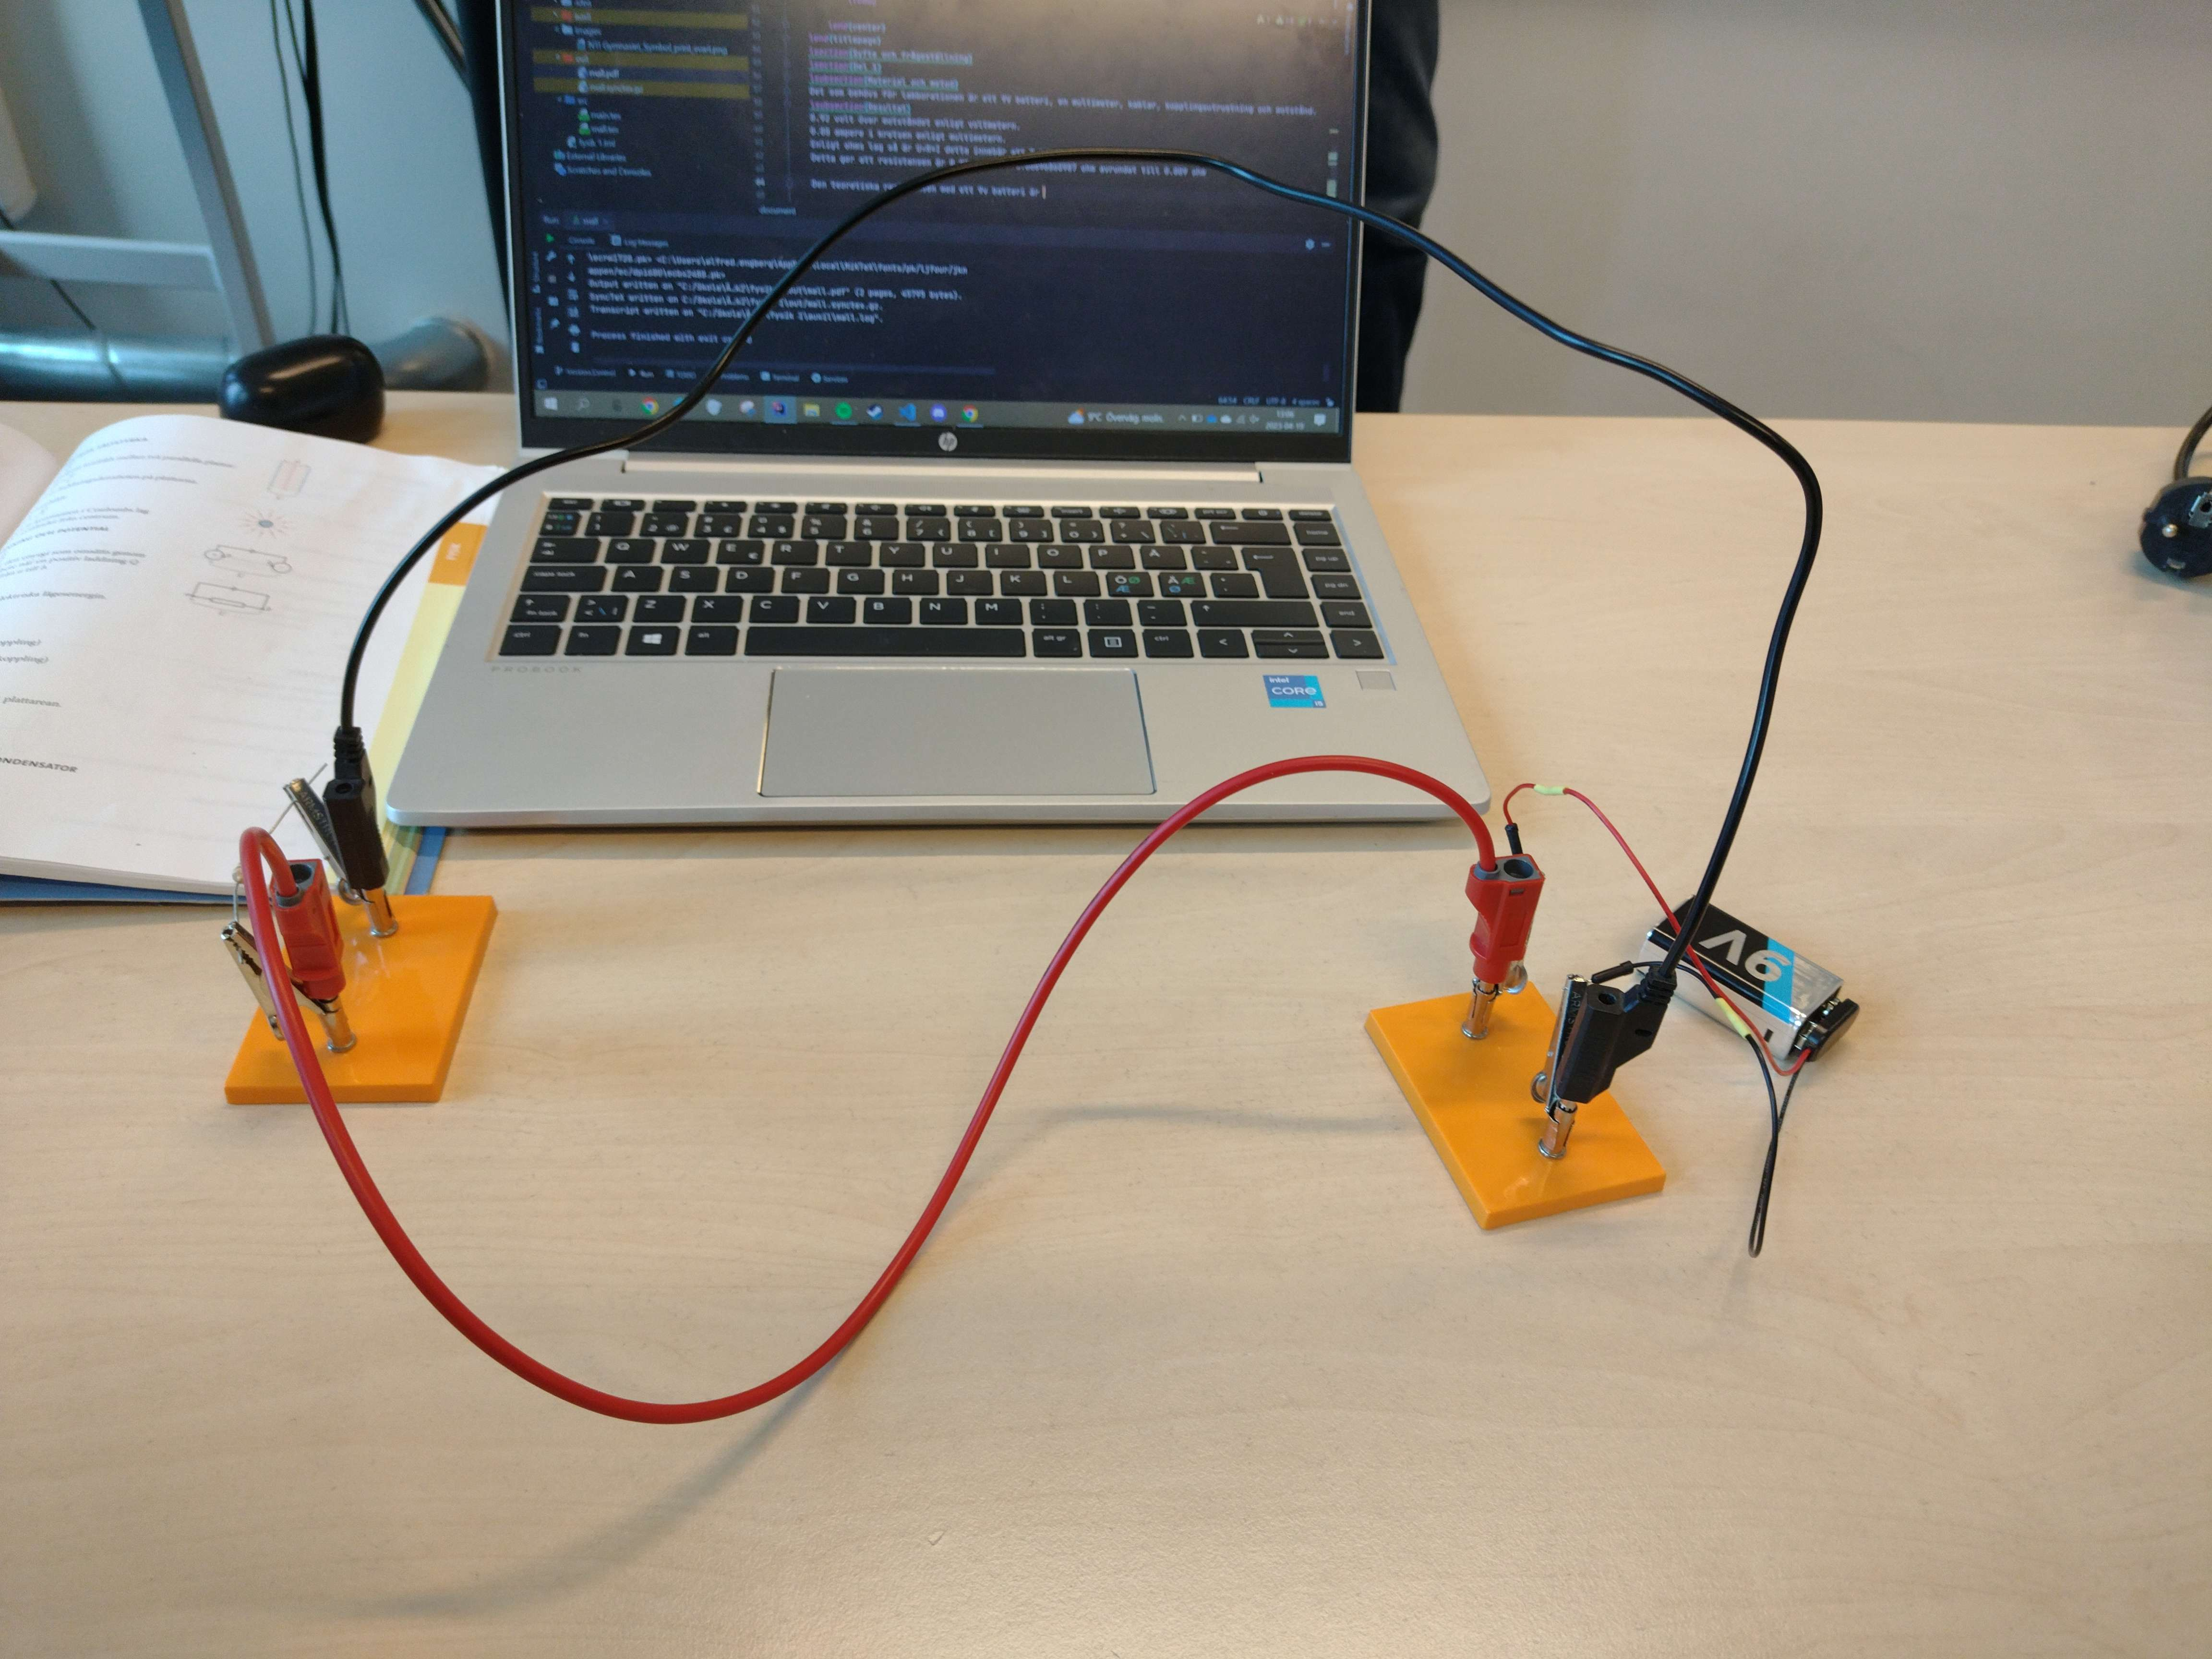
\includegraphics[width=0.4\textwidth]{../images/labb1.png}
    \subsection{Analys}
    Vi tar ohms lag och tar 8.9 genom 0.08 och får svaret 111.25 ohm
    8.9/0.08= 111.25Ω
    \section{Del 2}
    \subsection{Material och metod}
    1 batteri, 1 multimeter, två kablar, tre kopplingsplintar med två krokodilklämmor vardera samt två motstånd.
    Vi seriakopplar ett batteri med två mostånd och mäter ut spänningen och strömmen
    \subsection{Resultat}
    Spänningen över resistansen 4.4 V
    0.04 Ampere
    \subsection{Analys}
    Vi tar ohms lag och tar 4.4 genom 0.04 och vi får reslutatet 110 ohm
    4.4/0.04=110Ω
    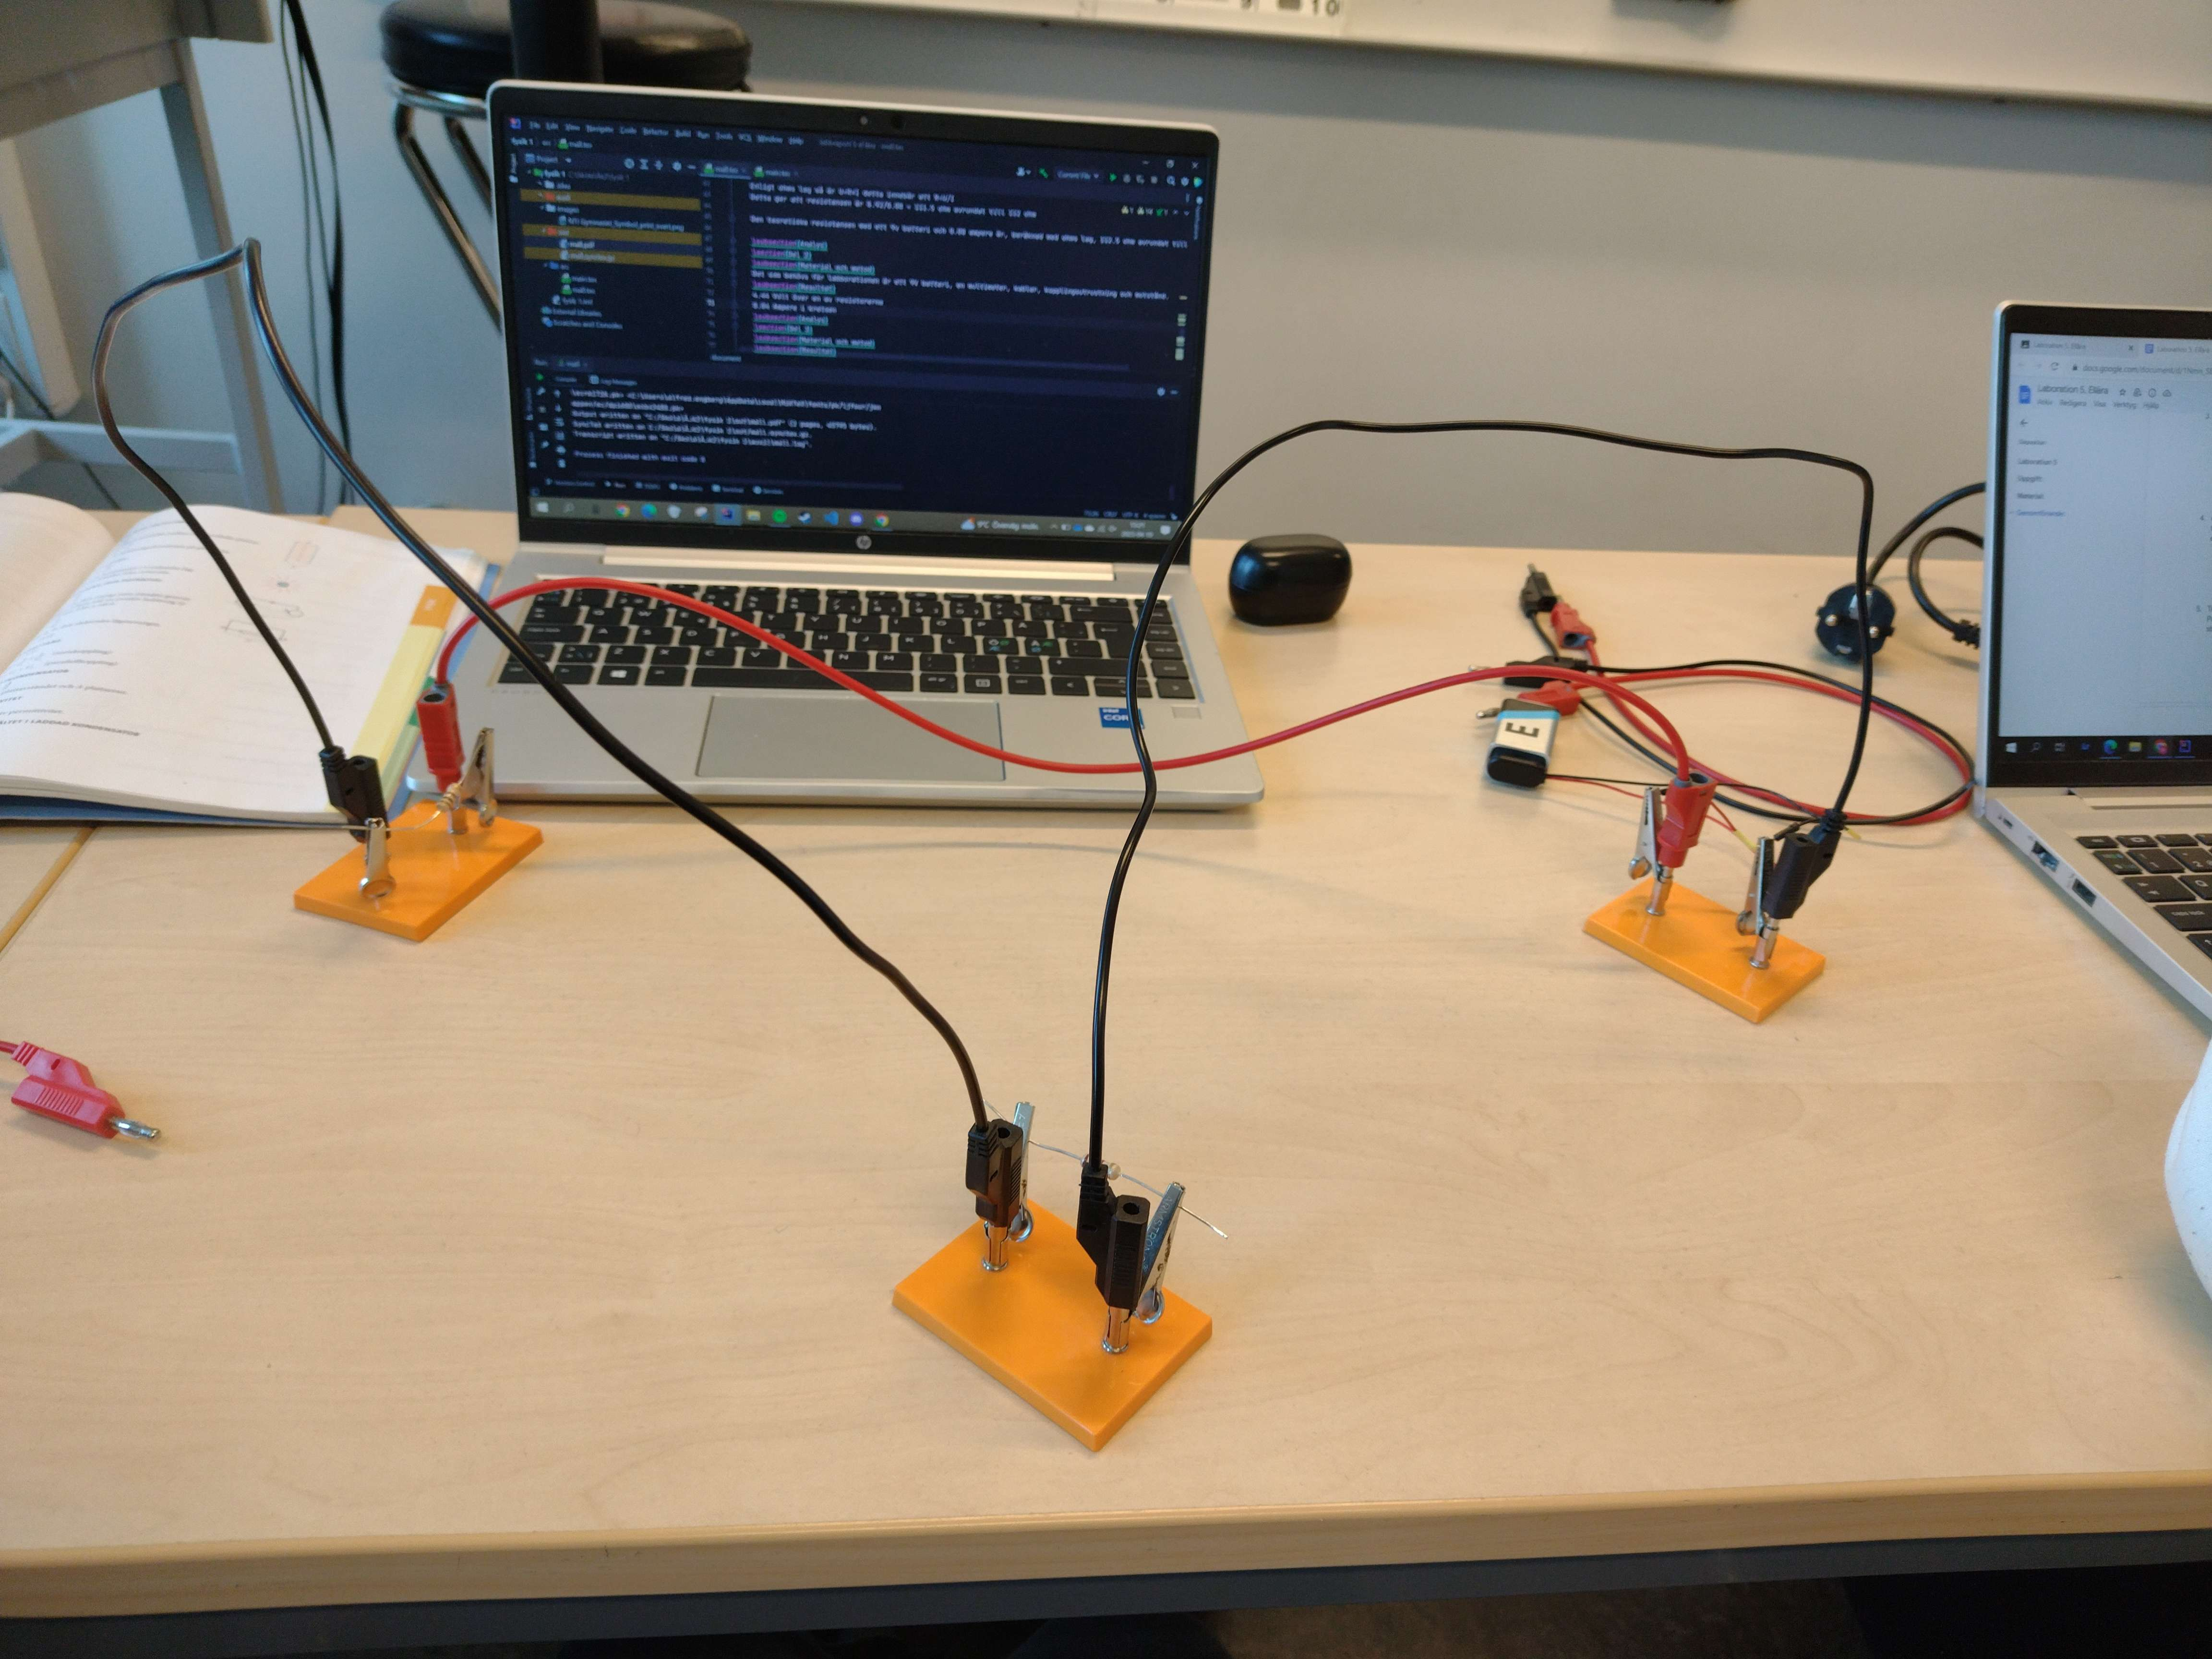
\includegraphics[width=0.4\textwidth]{../images/labb2.jpg}
    \section{Del 3}
    \subsection{Material och metod}
    1 batteri, 1 multimeter, två kablar, tre kopplingsplintar med två krokodilklämmor vardera samt två motstånd.
    Vi parkopplar resistorerna för att få redo på strömmen och spänning
    \subsection{Resultat}
    Spänningen över resistansen 8.3 V
    0.08 Ampere
    \subsection{Analys}
    Vi tar ohms lag och tar ohms lag och tar 8.3 genom 0.08 och då får vi resultatet 103.75 ohm
    8.3/0.08=103.75Ω
    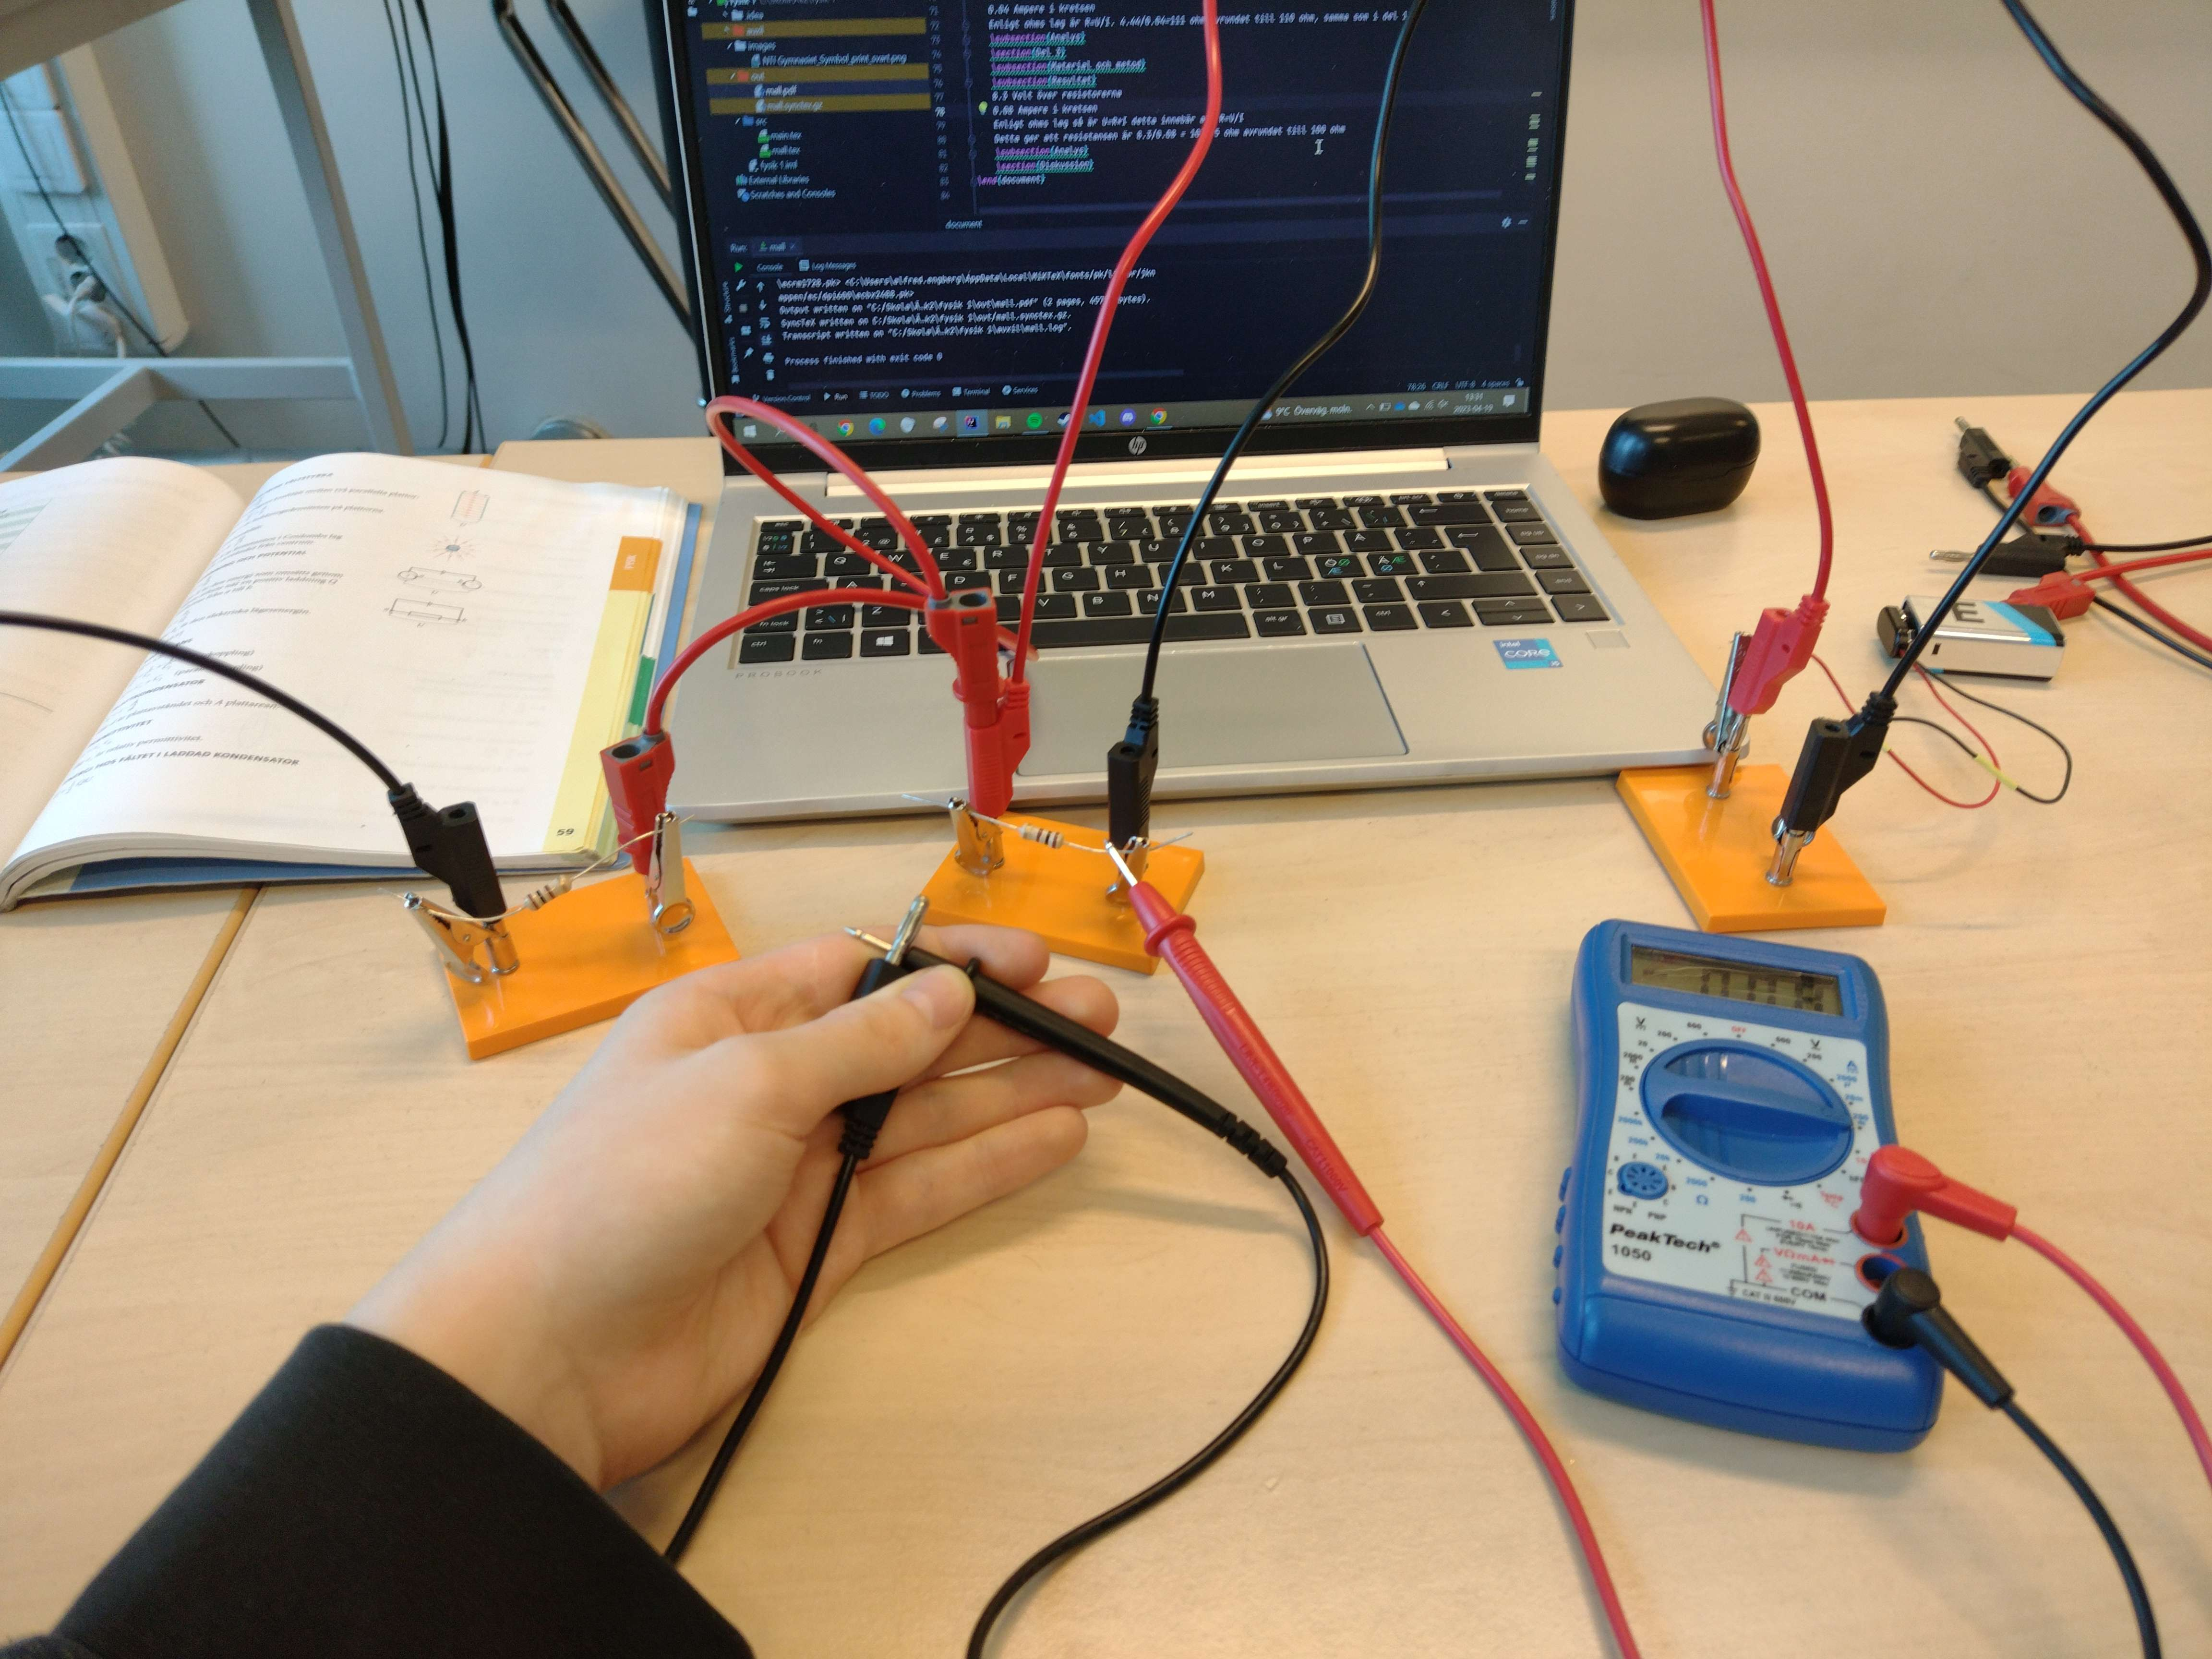
\includegraphics[width=0.4\textwidth]{../images/labb3.jpg}
    \section{Diskussion}
    Med hjälp av formalblad och min grups kunskaper om ellära gick labborationen endå bra. I början var det svårt att första vad som skulle kopplas till vad men i slutet gick allt ihop. Med allt vi vet så är rselutaten rimliga och värderna verkar stämma.
\end{document}
